\documentclass[border=10pt]{standalone}
\usepackage[T1]{fontenc}
\usepackage{tikz}
\usepackage{amsmath}

\definecolor{garnet}{HTML}{73000A}
\definecolor{atlantic}{HTML}{466A9F}
\definecolor{congaree}{HTML}{1F414D}
\definecolor{warmgrey}{HTML}{676156}
\definecolor{horseshoe}{HTML}{65780B}
\definecolor{rose}{HTML}{CC2E40}
\definecolor{honeycomb}{HTML}{A49137}
\definecolor{bk70}{HTML}{5C5C5C}
\definecolor{bk30}{HTML}{C7C7C7}

\begin{document}
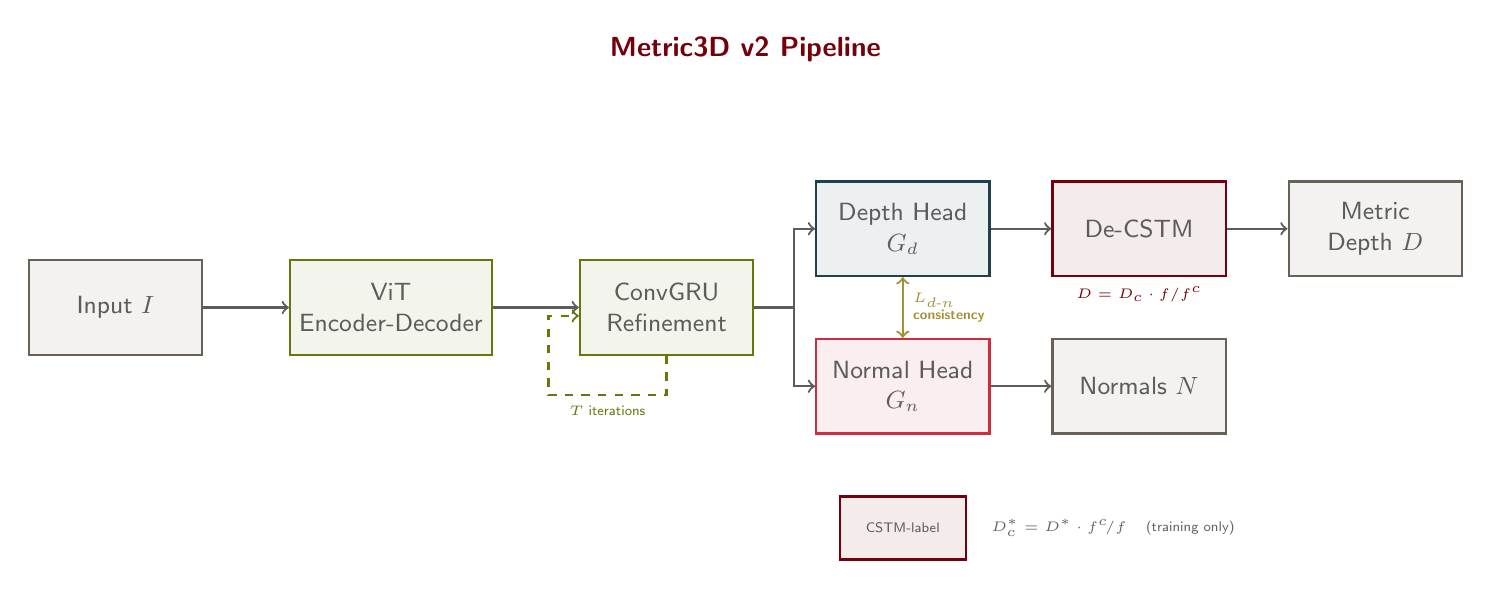
\begin{tikzpicture}[
    block/.style={
        draw=#1, thick, fill=#1!8,
        minimum height=1.2cm, minimum width=2.2cm,
        font=\sffamily\small, text=bk70, align=center,
    },
    arr/.style={->, thick, color=bk70},
    label/.style={font=\sffamily\tiny, text=warmgrey, align=center},
    newlabel/.style={font=\sffamily\tiny\bfseries, text=horseshoe, align=center},
]

% ── v2 Pipeline blocks ──
% Input
\node[block=warmgrey] (input) at (0, 0) {Input $I$};

% ViT Encoder-Decoder
\node[block=horseshoe] (backbone) at (3.5, 0) {ViT\\Encoder-Decoder};

% ConvGRU (new in v2)
\node[block=horseshoe] (gru) at (7, 0) {ConvGRU\\Refinement};

% ── Branch: Depth (top path) ──
\node[block=congaree] (dhead) at (10, 1.0) {Depth Head\\$G_d$};
\node[block=garnet] (decstm) at (13, 1.0) {De-CSTM};
\node[block=warmgrey] (dout) at (16, 1.0) {Metric\\Depth $D$};

% ── Branch: Normal (bottom path) ──
\node[block=rose] (nhead) at (10, -1.0) {Normal Head\\$G_n$};
\node[block=warmgrey] (nout) at (13, -1.0) {Normals $N$};

% ── Arrows: main trunk ──
\draw[arr] (input) -- (backbone);
\draw[arr] (backbone) -- (gru);

% ── Arrows: branch split ──
\draw[arr] (gru.east) -- ++(0.5, 0) |- (dhead.west);
\draw[arr] (gru.east) -- ++(0.5, 0) |- (nhead.west);

% ── Arrows: depth path ──
\draw[arr] (dhead) -- (decstm);
\draw[arr] (decstm) -- (dout);

% ── Arrows: normal path ──
\draw[arr] (nhead) -- (nout);

% ── ConvGRU iteration loop ──
\draw[arr, horseshoe, dashed] (gru.south) -- ++(0, -0.5) -- ++(-1.5, 0)
    node[midway, below, font=\sffamily\tiny, text=horseshoe] {$T$ iterations}
    |- ([yshift=-0.72cm]gru.north west);

% ── Consistency loss ──
\draw[<->, thick, honeycomb] (dhead.south) -- (nhead.north)
    node[midway, right, font=\sffamily\tiny\bfseries, text=honeycomb, align=left] {$L_{d\text{-}n}$\\consistency};



% ── CSTM-label annotation (training only) ──
\node[block=garnet, minimum width=1.6cm, minimum height=0.8cm, font=\sffamily\tiny]
    (cstm_label) at (10, -2.8) {CSTM-label};
\node[font=\sffamily\tiny, text=warmgrey, anchor=west] at (11, -2.8)
    {$D^*_c = D^* \cdot f^c\!/f$ \quad (training only)};

% ── De-CSTM note ──
\node[font=\sffamily\tiny, text=garnet, anchor=north] at (decstm.south)
    {$D = D_c \cdot f/f^c$};

% ── Title ──
\node[font=\sffamily\bfseries, text=garnet, anchor=south] at (8, 3.0) {Metric3D v2 Pipeline};


\end{tikzpicture}
\end{document}
